\chapter{Theoretical Background}\label{chapter:background} \

In Chapter~\ref{chapter:background} we will introduce the
background information that is required to understand
the main ideas of this thesis. First we introduce
the basic concepts of quantum computing. Then we will
describe advanced concepts regarding quantum noise. We
assume some baseline \ac{ml} knowledge, however, we
will provide an outlook into \ac{qml}. Finally, we
present several types of adversarial machine learning
and adversarial training as a defense mechanism. \

\section{Fundamentals of Quantum Computing} \

\subsection{Qubit}\label{subsection:qubit} \

The basic computing unit in quantum computing is the
\textit{qubit}~\cite{schumacher_quantum_1995}. Similar to the classical
bit, a qubit also has a state. While a bit has either a
\textit{0} or \textit{1} state, the qubit can have
many more states. The quantum equivalent to the classical
bit states would be \(\ket{0}\) and \(\ket{1}\) in Dirac
notation~\cite{dirac_new_1939} and they represent the orthonormal computational
basis states in Equation~\ref{eq:qubit_bases}. \

\begin{equation}\label{eq:qubit_bases}
    \ket{0} = \begin{pmatrix}
                1 \\ 0
              \end{pmatrix} \qquad \qquad
    \ket{1} = \begin{pmatrix}
                0 \\ 1
              \end{pmatrix}
\end{equation} \

What makes the qubit different and more capable than
the classical bit is that it can also have different states
created by a linear combination or \textit{superposition} from
its basis states. The linear combination in Equation
~\ref{eq:qubit_superposition} is the complete representation
of a qubit, where \(\alpha\) and \(\beta\) are two complex numbers that
are denominated \textit{probability amplitudes}.
The values \(\alpha\) and \(\beta\) represent a distribution, in which
with probability \(|\alpha|^2\) we will observe a \textit{0}
value and with probability \(|\beta|^2\) we will observe a
\textit{1} value. This distribution is determined by the
Born rule~\cite{born_quantenmechanik_1926} and states that \(|\alpha|^2 + |\beta|^2 \stackrel{!}{=} 1\).
The Born rule thus implies that a qubit state is a unitary vector in
a two-dimensional complex vector space. Although the
probability amplitudes can take on any complex value as long
as they fulfill the Born rule, when we perform a measurement
on the qubit it \textit{collapses} to one of the two basis
states. \

\begin{equation}\label{eq:qubit_superposition}
  \ket{\psi} = \alpha\ket{0} + \beta\ket{1}
\end{equation} \

In the real physical world qubits can be implemented by
several different small particles. However, the mathematical
qubit abstraction helps establish a baseline computing unit
for quantum computing independent of which particle it is
being represented by~\cite{nielsen_quantum_2010}. While in this perfect
mathematical description noise doesn't occur, there are
different mechanisms to represent the noise that quantum
computers suffer from, namely the density operator that will
be introduced in Subsection~\ref{subsection:density_operator}. \

\subsection{Bloch Sphere} \

The qubit state from Equation~\ref{eq:qubit_superposition} can be
rewritten into Equation~\ref{eq:qubit_global_phase}, where \(e\)
is the Euler number, \(i\) is the imaginary number, and \(\gamma\),
\(\varphi\), and \(\theta\) are real numbers. \

\begin{equation}\label{eq:qubit_global_phase}
  \ket{\psi} = e^{i\gamma} \left( \cos{\frac{\theta}{2}}\ket{0} + e^{i\varphi}\sin{\frac{\theta}{2}}\beta\ket{1} \right)
\end{equation} \

Because for a single qubit the global phase \(e^{i\gamma}\) has no
observable effects, we can omit it and write the state of a qubit as: \

\begin{equation}\label{eq:qubit_bloch}
  \ket{\psi} = \cos{\frac{\theta}{2}}\ket{0} + e^{i\varphi}\sin{\frac{\theta}{2}}\beta\ket{1}
\end{equation} \

where \(\theta\) and \(\varphi\) determine a point in the Bloch
sphere~\cite{bloch_nuclear_1946}. The Bloch sphere (Fig.~\ref{fig:bloch_sphere})
is a helpful visual representation for understanding the state of a
qubit. In Section~\ref{section:noise} this representation will be
utilized to show the effects of quantum noise on a quantum state. It
can also be used to visualize the effect of the operations performed
on quantum states, these operations are called \textit{gates} and 
they will be introduced in Subsection~\ref{subsection:gates}. \

\begin{figure}[ht]
  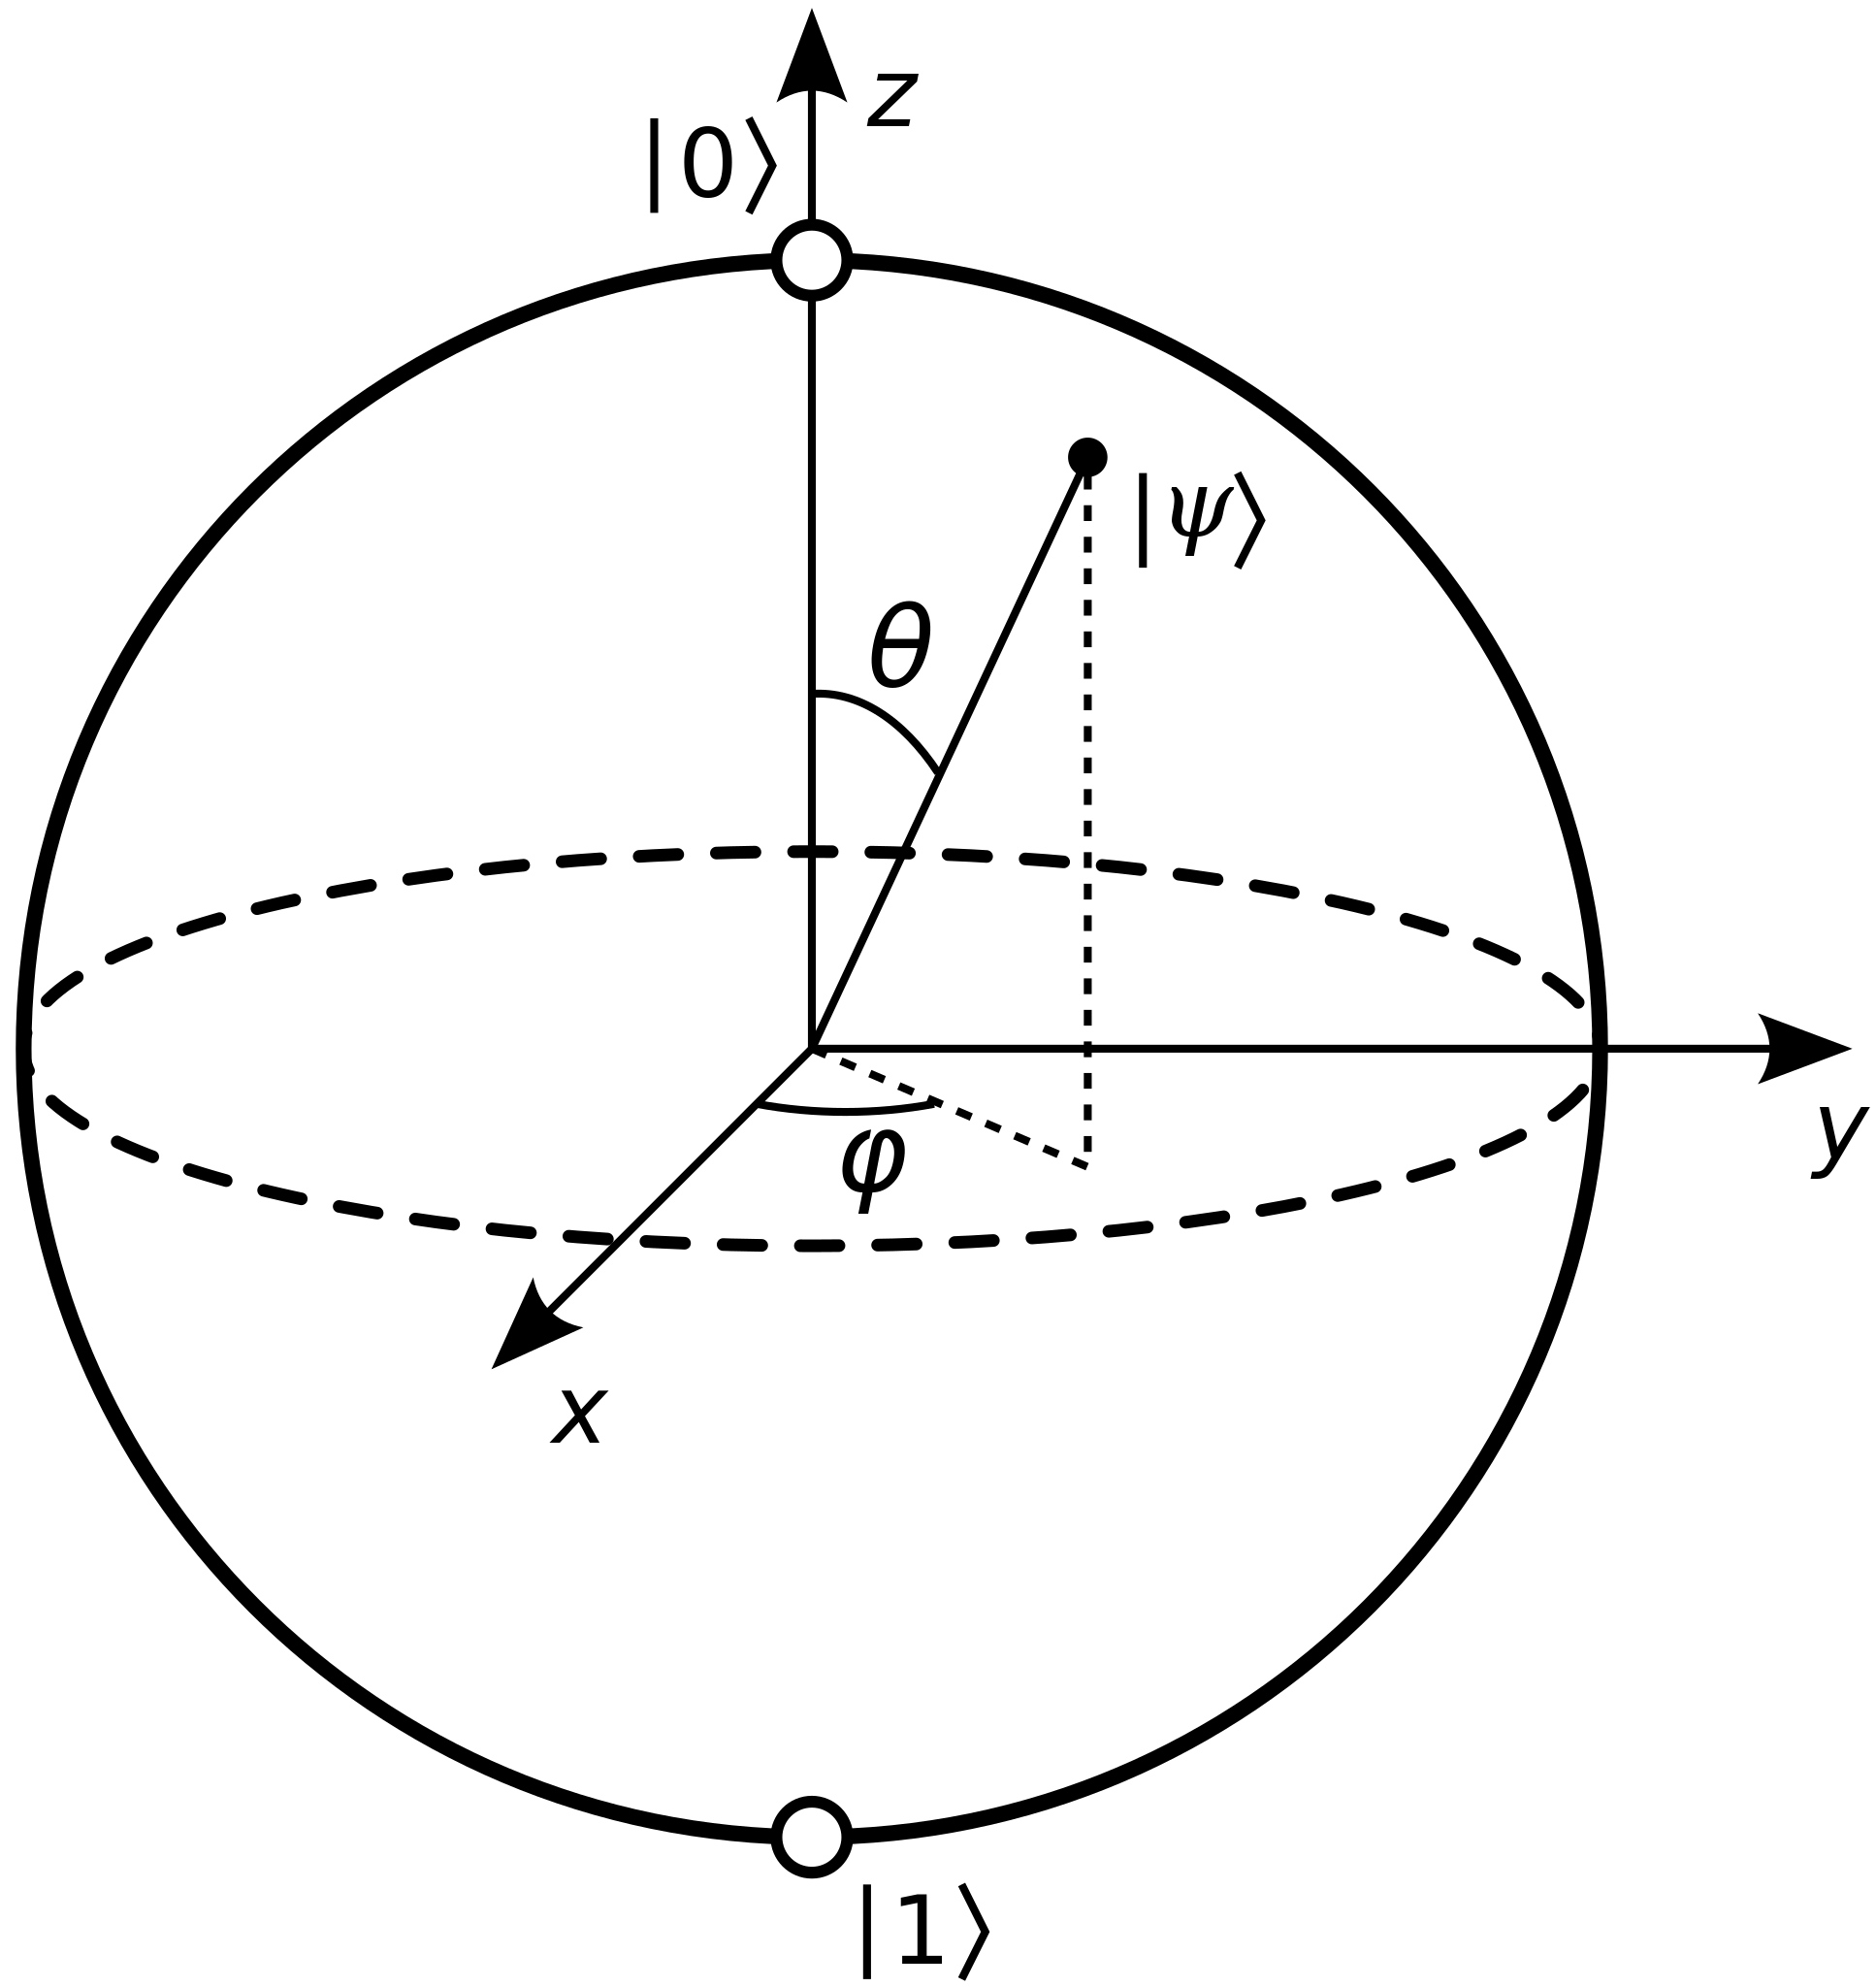
\includegraphics[scale=0.1]{figures/Bloch_sphere.png}
  \centering
  \caption{Bloch sphere representation of a qubit. Image taken from \href{https://commons.wikimedia.org/wiki/File:Bloch_Sphere.svg}{https://commons.wikimedia.org/wiki/File:Bloch\_Sphere.svg} under the \href{https://en.wikipedia.org/wiki/Creative_Commons}{Creative Commons Attribution-Share Alike 3.0 Unported license}.}
~\label{fig:bloch_sphere}
\end{figure} \

\subsection{Multiple qubits} \

To describe multiple qubits we utilize the fundamentals presented in
Subsection~\ref{subsection:qubit} and expand them. For two qubits
\(\ket{00}, \ket{01}, \ket{10}\), and \(\ket{11}\) are the computational basis.
A general representation for a two qubit system can be found in 
Equation~\ref{eq:two_qubits}, where all the probability amplitudes must
follow the Born rule. \ 

\begin{equation}\label{eq:two_qubits}
  \ket{\psi} = \alpha_{00}\ket{00} + \alpha_{01}\ket{01} + \alpha_{10}\ket{10} + \alpha_{11}\ket{11}
\end{equation} \

Due to the Born rule the measurement results for
\(x = \left\{00, 01, 10, 11\right\}\) follow the probability
distribution determined by \(|\alpha_{x}|^2\). Similar to a
single qubit, once a measurement on both qubits is performed,
the state of the qubits will collapse to the measured computational
basis. Nevertheless, with multiple qubits we are able to perform
measurements on a subset of qubits. In the case of a two-qubit
system, measuring the first qubit will collapse its value. However,
the second's qubit state will remain. In the case of Eq.~\ref{eq:two_qubits},
if \textit{0} was measured in the first qubit, the amplitudes \(\alpha_{10}\)
and \(\alpha_{11}\) would disappear from the state as they are no longer
possible. Furthermore, the remaining amplitudes must be normalized,
such as in Eq.~\ref{eq:measure_first}, to fulfill Born's rule.  \

\begin{equation}\label{eq:measure_first}
  \ket{\psi'} = \frac{\alpha_{00}\ket{00} + \alpha_{01}\ket{01}}
                    {\sqrt{|\alpha_{00}|^2 + |\alpha_{01}|^2}}
\end{equation} \

In Equation~\ref*{eq:multiple_qubits} we can find a general representation of
a set of \textit{n} qubits. For a system composed by \textit{n} qubits there are \(2^n\)
amplitudes. If we tried to simulate a quantum system with \(n = 50\), assuming
that complex numbers require 8 bytes to be stored~\cite{numpy}, a classical computer would need
approximately 9000 terabytes to store the generated quantum state. This simple calculation
shows the reason why quantum computers are so promising and also why classical computers
are not able to process quantum information efficiently. \
% (2**50)*8 = 9007199254740992
% https://docs.scipy.org/doc/numpy-1.17.0/user/basics.types.html

\begin{equation}\label{eq:multiple_qubits}
  \ket{\psi} = \alpha_{00}\ket{0\cdots0} + \cdots + \alpha_{2^{n-1}}\ket{1\cdots1}
\end{equation} \

\subsection{Quantum Gates}\label{subsection:gates}
- Introduce quantum gates \
    - Equate a gate with a unitary matrix \
    - Pauli Gates \
\begin{equation}\label{eq:pauli_x}
    X = \begin{pmatrix}
          0 & 1 \\
          1 & 0
        \end{pmatrix} \qquad \qquad
    \Qcircuit @C=1em @R=1em {
      & \gate{X} & \qw
    }
\end{equation} \

\begin{equation}\label{eq:pauli_y}
  Y = \begin{pmatrix}
        0 & -i \\
        i & 0
      \end{pmatrix} \qquad \qquad
  \Qcircuit @C=1em @R=1em {
    & \gate{Y} & \qw
  }
\end{equation} \

\begin{equation}\label{eq:pauli_z}
  Z = \begin{pmatrix}
        1 & 0 \\
        0 & -1
      \end{pmatrix} \qquad \qquad
  \Qcircuit @C=1em @R=1em {
    & \gate{Z} & \qw
  }
\end{equation} \

    - Hadamard Gate \
\begin{equation}\label{eq:hadamard}
  H = \frac{1}{\sqrt{2}} 
      \begin{pmatrix}
        1 & 1 \\
        1 & 1
      \end{pmatrix} \qquad \qquad
  \Qcircuit @C=1em @R=1em {
    & \gate{H} & \qw
  }
\end{equation} \

- Multiple qbits gates

\begin{equation}\label{eq:cnot}
  CNOT = \begin{pmatrix}
          1 & 0 & 0 & 0 \\
          0 & 1 & 0 & 0 \\
          0 & 0 & 0 & 1 \\
          0 & 0 & 1 & 0 \\
        \end{pmatrix} \qquad \qquad
  \Qcircuit @C=1em @R=1em {
      & \ctrl{1} & \qw \\
      & \targ & \qw \\
  }
\end{equation} \

\begin{equation}\label{eq:swap}
  SWAP = \begin{pmatrix}
          1 & 0 & 0 & 0 \\
          0 & 0 & 1 & 0 \\
          0 & 1 & 0 & 0 \\
          0 & 0 & 0 & 1 \\
        \end{pmatrix} \qquad \qquad
  \Qcircuit @C=1em @R=1em {
    & \qswap & \qw \\
    & \qswap \qwx & \qw \\
  }
\end{equation} \

- Introduce entanglement and bell states, 11,16 \
\begin{equation}\label{eq:entanglement}
  \Qcircuit @C=1em @R=1em {
    & \gate{H} & \ctrl{1} & \qw \\
    & \qw & \targ & \qw \\
  } \qquad \qquad
  \frac{1}{\sqrt{2}} \left(\ket{00} + \ket{11}\right)
\end{equation}

- Introduce quantum circuits \
- Introduce quantum measurement \
\subsection{Density Operator}\label{subsection:density_operator}
- Introduce the density operator \
- Introduce quantum algorithms* \

Todo:
- Citation for hadamard gate, pauli gate.

\section{Quantum Noise}\label{section:noise}
i.	Describe the types of noise that can occur.
ii.	Explain where can noise occur.
iii.	State how noise can be simulated.

\section{Quantum Machine Learning}
i.	Present the difference between QML and classical ML\@.
ii.	Introduce variational quantum circuits.
iii.	Explain quantum kernel methods.

\section{Adversarial Machine Learning}
i.	State generalization problems.
ii.	Present different attacks such as FGSM, C\&W, and PGD\@.
iii.	Introduce adversarial training as defence mechanism against adversarial attacks.
iv.	Explain the relationship between general accuracy and adversarial resilience.